\documentclass[a4paper,11pt]{article}
\usepackage{amsmath,amsthm,amsfonts,amssymb,amscd,amstext,vmargin,graphics,graphicx,tabularx,multicol} 
\usepackage[francais]{babel}
\usepackage[utf8]{inputenc}  
\usepackage[T1]{fontenc} 
\usepackage{pstricks-add,tikz,tkz-tab,variations}
\usepackage[autolanguage,np]{numprint} 

\setmarginsrb{1.5cm}{0.5cm}{1cm}{0.5cm}{0cm}{0cm}{0cm}{0cm} %Gauche, haut, droite, haut
\newcounter{numexo}
\newcommand{\exo}[1]{\stepcounter{numexo}\noindent{\bf Exercice~\thenumexo} : \marginpar{\hfill /#1}}
\reversemarginpar


\newcounter{enumtabi}
\newcounter{enumtaba}
\newcommand{\q}{\stepcounter{enumtabi} \theenumtabi.  }
\newcommand{\qa}{\stepcounter{enumtaba} (\alph{enumtaba}) }
\newcommand{\initq}{\setcounter{enumtabi}{0}}
\newcommand{\initqa}{\setcounter{enumtaba}{0}}

\newcommand{\be}{\begin{enumerate}}
\newcommand{\ee}{\end{enumerate}}
\newcommand{\bi}{\begin{itemize}}
\newcommand{\ei}{\end{itemize}}
\newcommand{\bp}{\begin{pspicture*}}
\newcommand{\ep}{\end{pspicture*}}
\newcommand{\bt}{\begin{tabular}}
\newcommand{\et}{\end{tabular}}
\renewcommand{\tabularxcolumn}[1]{>{\centering}m{#1}} %(colonne m{} centrée, au lieu de p par défault) 
\newcommand{\tnl}{\tabularnewline}

\newcommand{\bmul}[1]{\begin{multicols}{#1}}
\newcommand{\emul}{\end{multicols}}

\newcommand{\trait}{\noindent \rule{\linewidth}{0.2mm}}
\newcommand{\hs}[1]{\hspace{#1}}
\newcommand{\vs}[1]{\vspace{#1}}

\newcommand{\N}{\mathbb{N}}
\newcommand{\Z}{\mathbb{Z}}
\newcommand{\R}{\mathbb{R}}
\newcommand{\C}{\mathbb{C}}
\newcommand{\Dcal}{\mathcal{D}}
\newcommand{\Ccal}{\mathcal{C}}
\newcommand{\mc}{\mathcal}

\newcommand{\vect}[1]{\overrightarrow{#1}}
\newcommand{\ds}{\displaystyle}
\newcommand{\eq}{\quad \Leftrightarrow \quad}
\newcommand{\vecti}{\vec{\imath}}
\newcommand{\vectj}{\vec{\jmath}}
\newcommand{\Oij}{(O;\vec{\imath}, \vec{\jmath})}
\newcommand{\OIJ}{(O;I,J)}


\newcommand{\reponse}[1][1]{%
\multido{}{#1}{\makebox[\linewidth]{\rule[0pt]{0pt}{20pt}\dotfill}
}}

\newcommand{\titre}[5] 
% #1: titre #2: haut gauche #3: bas gauche #4: haut droite #5: bas droite
{
\noindent #2 \hfill #4 \\
#3 \hfill #5

\vspace{-1.6cm}

\begin{center}\rule{6cm}{0.5mm}\end{center}
\vspace{0.2cm}
\begin{center}{\large{\textbf{#1}}}\end{center}
\begin{center}\rule{6cm}{0.5mm}\end{center}
}



\begin{document}
\pagestyle{empty}
\titre{Contrôle 3 : Additions, soustractions et les cercles }{Nom :}{Prénom :}{Classe}{Date}

\vspace*{0.2cm}

\textbf{Les exercices avec un 
\includegraphics[scale=0.4]{trefle.eps} sont à faire sur la copie double.}\\


\begin{tabular}{|m{11cm}|c|c|c|}
\hline 
\textbf{Compétences} & \textbf{Acquis} & \textbf{En cours}  & \textbf{Non acquis} \\ 
\hline 
-Connaître le vocabulaire lié au cercle &  &  & \\
\hline
- Maîtriser le calcul en colonne &  &  &  \\ 
\hline 
-Maîtriser le calcul en ligne &  &  &  \\ 
\hline
-Établir un ordre de grandeur d'une somme ou d'une
différence &  &  &  \\ 
\hline 
-Construire, à la règle et au compas, un triangle 
connaissant les longueurs de ses côtés. &  &  &  \\ 
\hline
\end{tabular} 



\vspace*{0.5cm}

\exo{5} 
\includegraphics[scale=0.4]{trefle.eps} Cours

\q Donner la définition d'une différence.\\

\q Donner la définition d'un rayon.\\

\q A l'aide la figure ci-contre, recopier et compléter les phrases avec l'un des mots de la liste : une extrémité – le centre – le milieu – une corde –   un diamètre – cercle – disque.\\

\bmul{2}

\bi
\item Le point O est . . . du cercle.\\
	
\item $[AB]$ est . . . du cercle.\\

\item D appartient au . . .\\

\item Le point O est . . . du segment [OB]\\

\item Le point O est . . . du segment [AM]\\

\item $[AM]$ est . . . du cercle\\

\item B appartient au . . .\\
\ei

\columnbreak

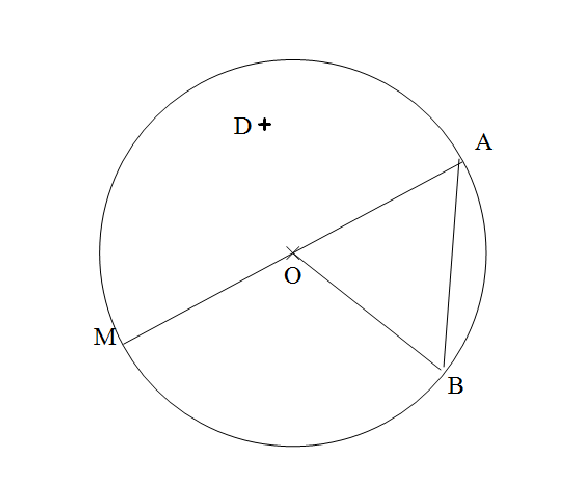
\includegraphics[scale=0.8]{cercle.eps} 


\emul

\vspace*{0.2cm}

\exo{2}
\includegraphics[scale=0.4]{trefle.eps} \\
Poser et effectuer les opérations suivantes :               

\bmul{2}

294,75 + 4347,53

\columnbreak

213,9 - 86,23	


\emul

\vspace*{0.2cm}

\exo{2} 
\includegraphics[scale=0.4]{trefle.eps}\\
 Calculer astucieusement avec la méthode vue en cours:

\bmul{2}

G = 1,4 + 75 + 18.60 + 125 \\

\columnbreak

 R = 5,125 + 21 + 4,7 + 9 + 2,3 + 0,875 + 34\\

\emul

\vspace*{0.2cm}

\exo{4} \\
Entourer en bleu, pour chaque calcul, le meilleur ordre de grandeur :\\

\begin{tabular}{|c|c|c|c|c|}
\hline 
9,85 + 2,86 + 1,18 $\approx$& 10 & 15 & 14 & 20 \\ 
\hline 
489,45 + 968,90 + 204 + 75,90 $\approx$& 1 000 & 1 800 & 2 000 &  3 000 \\ 
\hline 
143,2 – 98,7 $\approx$ & 40 & 45 & 50 & 245 \\ 
\hline 
345,56 - 129,56 $\approx$& 200 & 480 & 210 &  230 \\ 
\hline 
\end{tabular} 

\newpage

\exo{2}
\includegraphics[scale=0.4]{trefle.eps}\\
Angèle et Élise ont reçu chacune la même somme d'argent de leur grand-mère.\\
Angèle, qui possédait 34,65 euros, a maintenant 100 euros. 
Élise, quant à elle, possédait 48,50 euros.\\
Combien Élise a-t-elle d'argent maintenant ?\\

\vspace*{0.2cm}

\exo{2}
Sur la figure ci-dessous, tracer : \\
- 	le cercle de centre A et de rayon 2 cm ;\\
-	le cercle de centre K passant par B ;\\
-	le cercle de centre L et de diamètre 4 cm ;\\
-	le cercle de diamètre [NT].\\

\begin{flushleft}
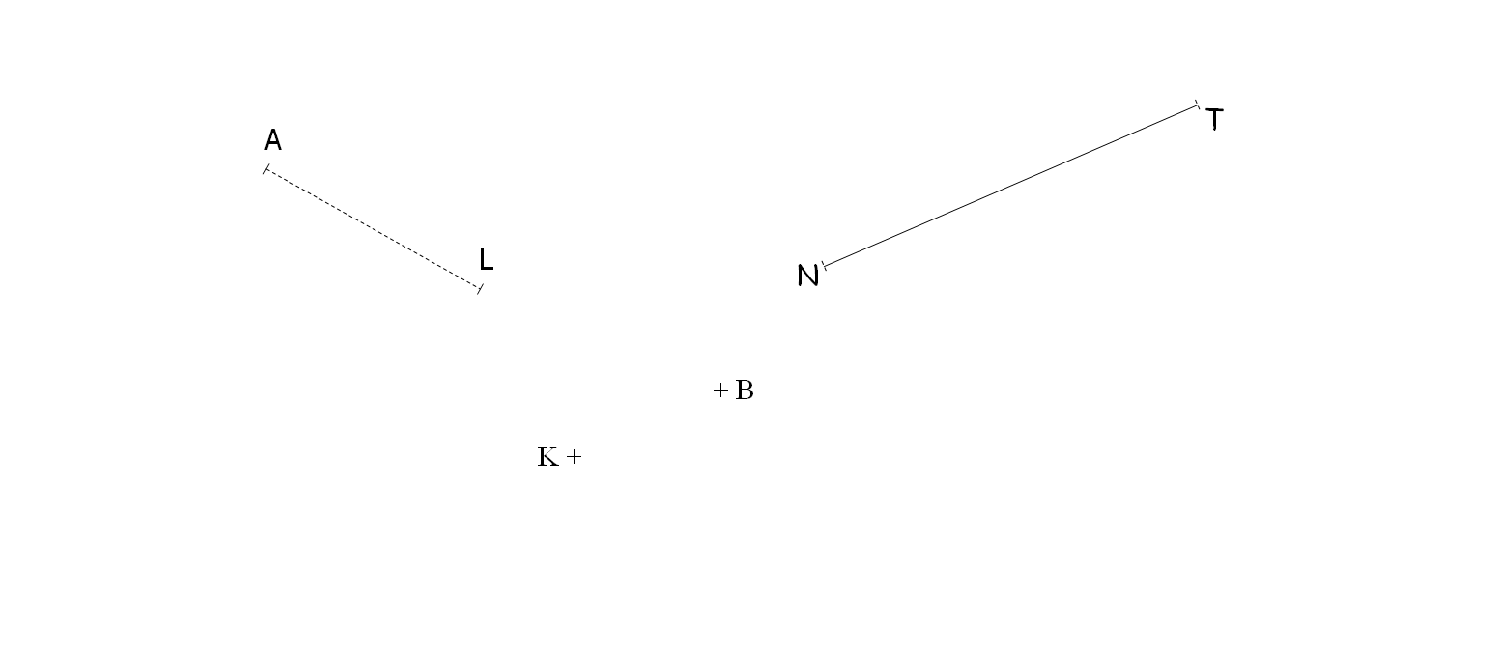
\includegraphics[scale=0.8]{cercle2.eps} 
\end{flushleft}



\exo{3}
\includegraphics[scale=0.4]{trefle.eps}\\
Construire soigneusement la figure ci-dessous en vraie grandeur.\\

\begin{center}
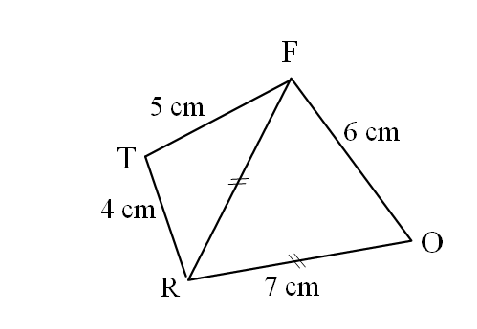
\includegraphics[scale=0.8]{triangles.eps} 
\end{center}


\exo{}Bonus\\
Sur le terrain de pétanque représenté par le rectangle ci-contre, Marc (placé en M) lance le cochonnet entre 6 m et 10 m.\\ 
Colorer en bleu la zone dans laquelle Marc peut lancer le cochonnet.\\

\begin{center}
\includegraphics[scale=0.65]{bonus1.eps} 
\end{center}








\end{document}
